%%
%% KCGS journal latex format example.
%% There are several options in this file, 
%% PLEASE READ THE FOLLOWING LINES BEFORE YOU USE.
%% 1. If you use KC2007 instead of MikTeX, use ``kotex'' package.
%% 2. If you don't have ``ifpdf'' package, 
%%    then use ``epsfig'' and ``epstopdf'' packages.
%%    (But usually you should have ``ifpdf'' package, 
%%    because the package is used in siggraph class.
%% 3. If you don't have ``caption'' package, 
%%    comment out "\usepackage[labelfont=bf]{caption}" command.
%% 4. There are several commands for squeezing figures and tables into a page.
%%    Uncomment those commands if you want to use them.
%% This file is tested under KC2008 and MikTex 2.4~2.5 with HLaTeX.
%%
%% If you have problems in using LaTeX, visit http://www.ktug.or.kr
%%
%% - 1st version 2007/08/22 Hyunjun Lee.
%% - 2nd version 2009/03/11 Hyunjun Lee.
%%   email: crowlove@postech.ac.kr
%%   Please do not email me if you have any questions or problems :)
%%

\documentclass[a4paper,twocolumn]{article}

%---------------------------------------------------------------------------
%% If you don't really know latex commands and changes you want to make,
%% you don't need to change anything up to "document begins" below.

\usepackage[hangul]{kotex}
\usepackage{dhucs-cmap}

%% Geometry package for page layout.
\usepackage{geometry}
\geometry{width=190mm, height=247mm, hmargin={1cm, 1cm}, vmargin={3cm, 2cm}}

%% We use one-half spacing.
\usepackage{setspace}
\onehalfspacing

%% Package to use both korean and english titles, authors, abstracts.
\usepackage{kcgs_utf}

%% The 'helvet' and 'times' packages define the typefaces used for
%% serif and sans serif type in this document. Computer Modern Roman 
%% is used for mathematics typesetting. The scale factor is set to .92
%% to bring the sans-serif type in line with the serif type.
\usepackage[scaled=.92]{helvet}
\usepackage{times}

%% The 'graphicx' package allows for the inclusion of EPS figures.
\usepackage{ifpdf}
	\ifpdf % compile with pdflatex
		\usepackage[pdftex]{graphicx}
	\else % latex => compile with dvipdfmx
		\usepackage{graphicx}
			\DeclareGraphicsExtensions{.jpg,.pdf,.png,.eps}
			\DeclareGraphicsRule{.jpg}{eps}{.bb}{}
			\DeclareGraphicsRule{.pdf}{eps}{.bb}{}
			\DeclareGraphicsRule{.png}{eps}{.bb}{}
	\fi

%% Or, if you don't have ``ifpdf'' package, use this two packages instead.
%\usepackage{epsfig}
%\usepackage{epstopdf}

%% Remove '제','절' from section names.
\kscntformat{section}{}{.}

%% Optional: the 'caption' package provides a nicer-looking replacement
%% for the standard caption environment. With 'labelfont=bf,'textfont=it',
%% caption labels are bold and caption text is italic.
%% You don't have to use this package if the package does not exist.
%\usepackage[labelfont=bf]{caption}

%% Uncomment following lines if you want to squeeze figures and tables into a page.
%\renewcommand{\topfraction}{0.95}
%\setcounter{bottomnumber}{1}
%\renewcommand{\bottomfraction}{0.95}
%\setcounter{totalnumber}{3}
%\renewcommand{\textfraction}{0.05}
%\renewcommand{\floatpagefraction}{0.95}
%\setcounter{dbltopnumber}{2}
%\renewcommand{\dbltopfraction}{0.95}
%\renewcommand{\dblfloatpagefraction}{0.95}

%---------------------------------------------------------------------------
% document begins

\begin{document}

%% Title.
\title{Sparse Ellipsometry: 비구조화 플래시 사진을 이용한 편광 SVBRDF 및 형상의 휴대용 취득법\footnote{
		구두 발표 논문}
	\footnote{
		본 논문은 요약 논문이며, ACM SIGGRAPH 2022에서 발표 예정임.}
}

%% Author names.
\author{황인승$^{1\circ}$
\and 전석준$^{1}$
\and Adolfo Muñoz$^{3}$
\and Diego Gutierrez$^{3}$
\and Xin Tong$^{2}$
\and 김민혁$^{1*}$}

\affiliation{$^{1}$KAIST 
	\hspace{5mm} $^{2}$Microsoft Research Asia 
	\hspace{5mm} $^{3}$Universidad de Zaragoza - I3A}

\authoremail{
	$^{1}$\{ishwang, sjjeon, minhkim\}@vclab.kaist.ac.kr \hspace{5mm}
	$^{2}$xtong@microsoft.com \hspace{5mm}
	$^{3}$\{adolfo, didgog\}@unizar.es}

%% English title.
\entitle{Sparse Ellipsometry: Portable Acquisition of Polarimetric SVBRDF	and Shape with Unstructured Flash Photography}

%% English author names.
\enauthor{Inseung Hwang$^{1\circ}$
	\and Daniel S. Jeon$^{1}$
	\and Adolfo Muñoz$^{3}$
	\and Diego Gutierrez$^{3}$
	\and Xin Tong$^{2}$
	\and Min H. Kim$^{1*}$}

\enaffiliation{$^{1}$KAIST 
	\hspace{5mm} $^{2}$Microsoft Research Asia 
	\hspace{5mm} $^{3}$Universidad de Zaragoza - I3A}

% (Optional) Teaser
%\teaser{
%  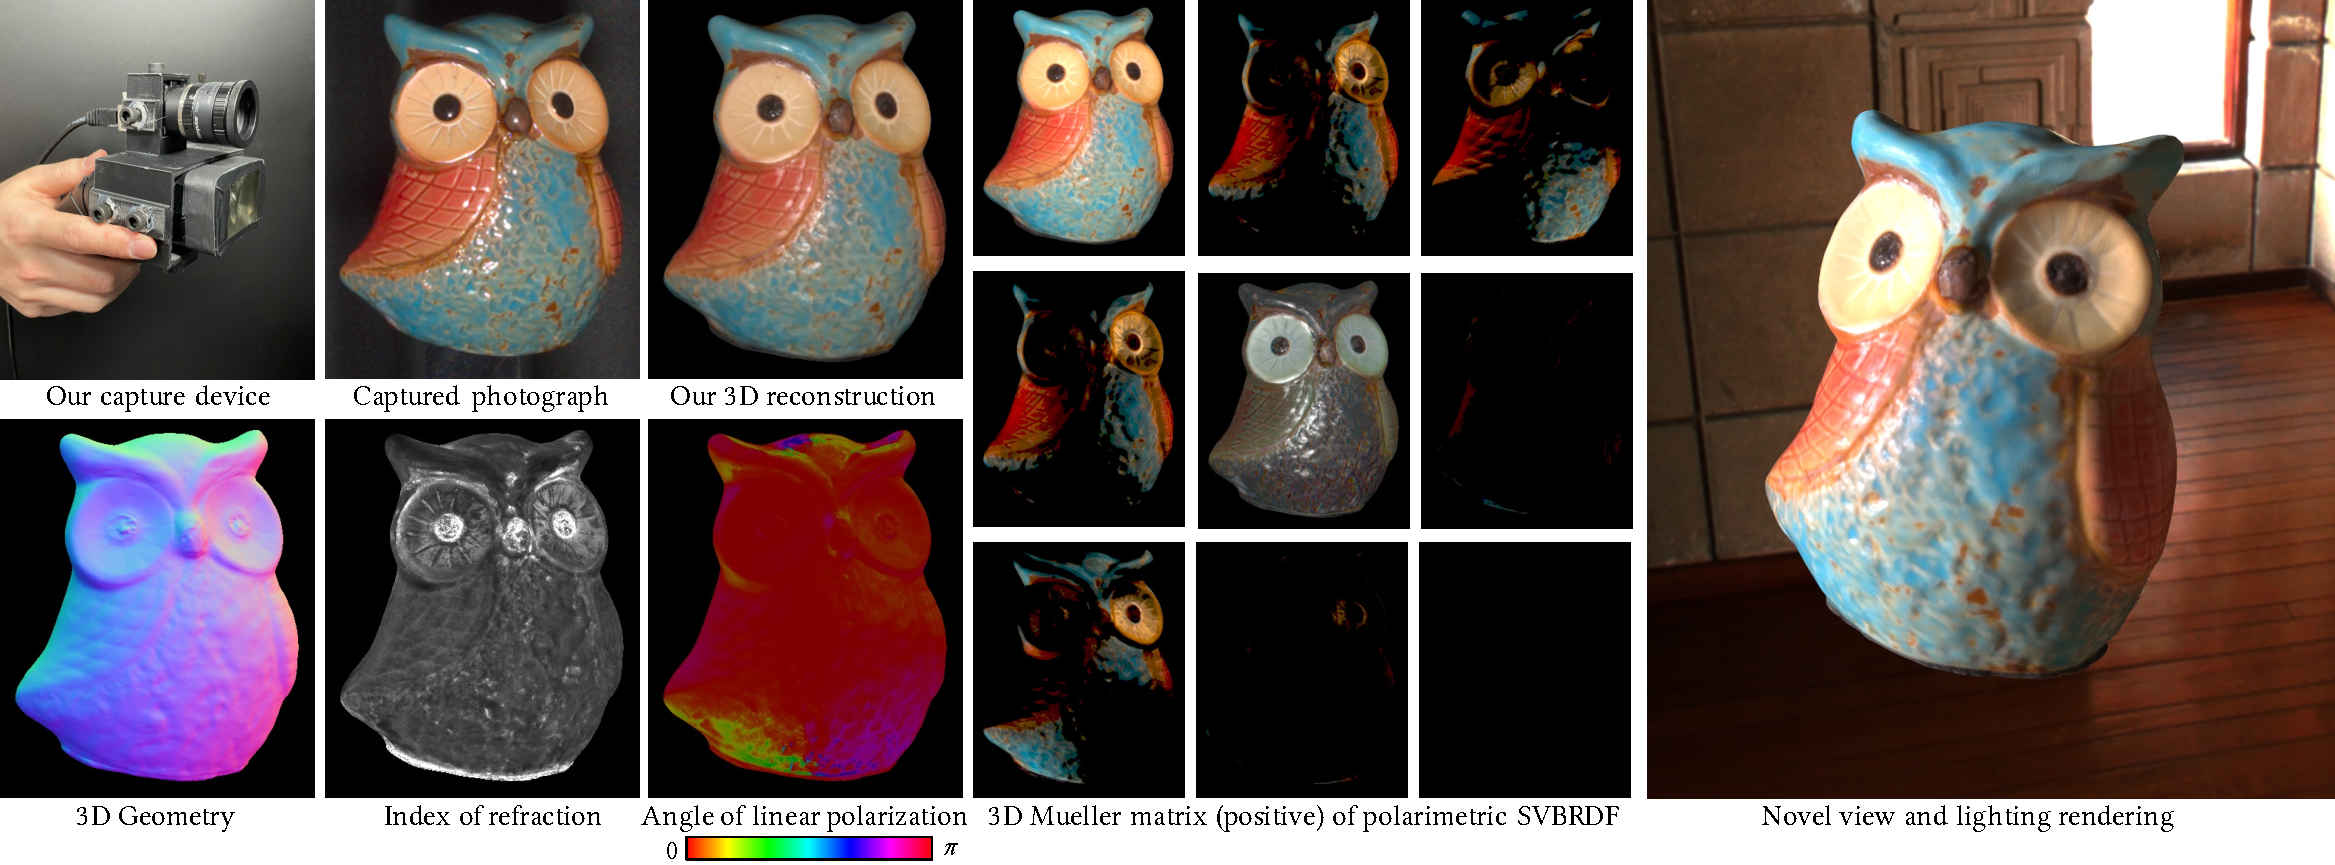
\includegraphics[width=0.95\textwidth]{fig/teaser.pdf}
%  \caption{본 연구의 촬영 시스템 및 복원 결과물, 3D 뮐러 행렬, 그리고 가상의 시점 및 광원 렌더링 결과물.}
%  \label{fig:teaser}
%}

%% Abstract.


%% English abstract.
%\begin{enabstract}
%
%The ``Abstract'' title should be written in (bold, 14pt) font size and contents should be written in (10pt).
%Please write abstract of the paper.
%
%\end{enabstract}

%% Keywords that describe your work.
%\keywords{편광 모습, 3D 재건, 물질 모습, 형상}
%\enkeywords{Polarimetric appearance, 3D reconstruction,	material appearance, shape}

%% The ``\maketitle'' command should be excuted after abstract section and keywords are written.
\let\footnote\thanks
\maketitle

%---------------------------------------------------------------------------
% paper begins
%\footnote*{
%	구두 발표 논문
%}

%\begin{abstract}
\section*{요약}
\label{sec:abstrct}
	편광해석법(Ellipsometry)을 사용하면 물질의 편광 정보를 측정할 수 있으나 다양한 구성의 조명과 센서로 구성된 광학 부품의 정밀한 회전을 요구한다. 
	%이로 인해 실험실 조건에서 정밀하게 캘리브레이션된 복잡한 촬영 장치에서 생성되며 일반적으로 오브젝트당 며칠 정도의 매우 긴 촬영 시간이 소요된다. 
	%최근의 기술을 사용하면 편광의 공간적으로 변화하는(spatially-varying) 반사율 정보를 촬영할 수 있지만 단일 시점으로 제한되거나 모든 시점을 촬영할 수 있지만 오브젝트가 단일 균질 물질로 만들어진 구형 물체로 제한된다. 
	본 연구는 편광 SVBRDF와 3D 형상을 동시에 촬영하는 휴대용 편광 획득 방법인 Sparse ellipsometry를 소개한다. 
	%우리의 휴대용 장치는 기성품의 고정 광학 부품으로 구성되어 있다. 총 촬영 시간은 며칠이 아닌 개체당 20분에서 30분 사이이다. 
	본 연구는 확산 및 반사 구성 요소와 단일 산란을 포함하는 완전한 편광 SVBRDF 모델을 개발하고 생성 모델링을 통한 반사 샘플의 데이터 증강을 사용하여 새로운 편광 인버스 렌더링(inverse rendering) 알고리즘을 제안한다. 연구 결과는 실제 객체의 캡처된 편광 BRDF의 최근 실측 데이터셋과 일치함을 보여준다.
	
%\end{abstract}

\section{서론}
\label{sec:introduction}
실제 객체의 BRDF(양방향 반사율 분포 함수)의 사실적인 모델링은 물리 기반 렌더링의 핵심 기술이다.
그러나 빛의 편광 상태에 대한 산란 효과는 인간의 눈으로 대부분의 경우 감지할 수 없기 때문에 일반적으로 무시되었다.
그러나 편광은 광학 센서로 쉽게 촬영할 수 있으며 물체의 기하 및 물질 속성에 대한 유용한 정보를 제공한다.

%편광해석법은 광학 측정을 사용하여 물질과의 상호 작용이 입사광의 편광 상태를 변경하는 방식을 특정한다~\cite{azzam2016stokes}. 
%최근의 이미지 기반 편광해석법에는 두 가지 주요 접근 방식이 있다. 실제 물체의 편광 SVBRDF를 캡처할 수 있지만 단일 시점으로 제한되는 방식과~\cite{Baek2018} 편광 정보를 모든 시야 방향에서 측정할 수 있지만 하나의 균질한 단일 물질로 구성된 구형 물체로 제한되는 방식이 있다~\cite{Baek2020}. 
%최근의 기술을 사용하면 편광의 공간적으로 변화하는(spatially-varying) 반사율 정보를 촬영할 수 있지만 단일 시점으로 제한되거나 모든 시점을 촬영할 수 있지만 오브젝트가 단일 균질 물질로 만들어진 구형 물체로 제한된다.
%또한 며칠 정도의 긴 촬영시간을 요구하며 정교한 광학 테이블 구성과 회전하는 광학 장비가 필요하다.
본 연구는 임의의 기하구조뿐만 아니라 모든 시점 방향에서 공간적으로 변하는 편광 물체를 동시에 촬영할 수 있는 최초의 연구이다. 기성품의 편광 카메라와 회전 요소가 필요 없는 선형 편광판이 달린 플래시라이트를 결합한 휴대용 장치를 이용한다. 
실제 데이터와 정확하게 일치하는 결과물을 내며 촬영 시간은 기존 접근 방식의 며칠이 아닌 20분에서 30분 사이이다.

구조화되지 않은 희박하게 촬영된 이미지 세트에서 인버스 렌더링을 포함하는 최적화 알고리즘을 사용하여 편광 반사율과 3D 모양을 복원한다. 
난반사 및 정반사뿐만 아니라 단일 산란도 포함된 새로운 편광 SVBRDF 모델을 제안하며, 최근 연구의 실제 데이터셋을 통해 일치함을 확인한다.
매우 좁은 정반사 로브의 경우 정반사 파라미터를 추정하기 충분하지 않기 때문에, 새로운 합성 시점으로 입력을 증강하는 생성 모델링 전략을 제안한다.


\begin{figure*}[tpb]
	\vspace{-2mm}%
	\centering%
	\footnotesize%
	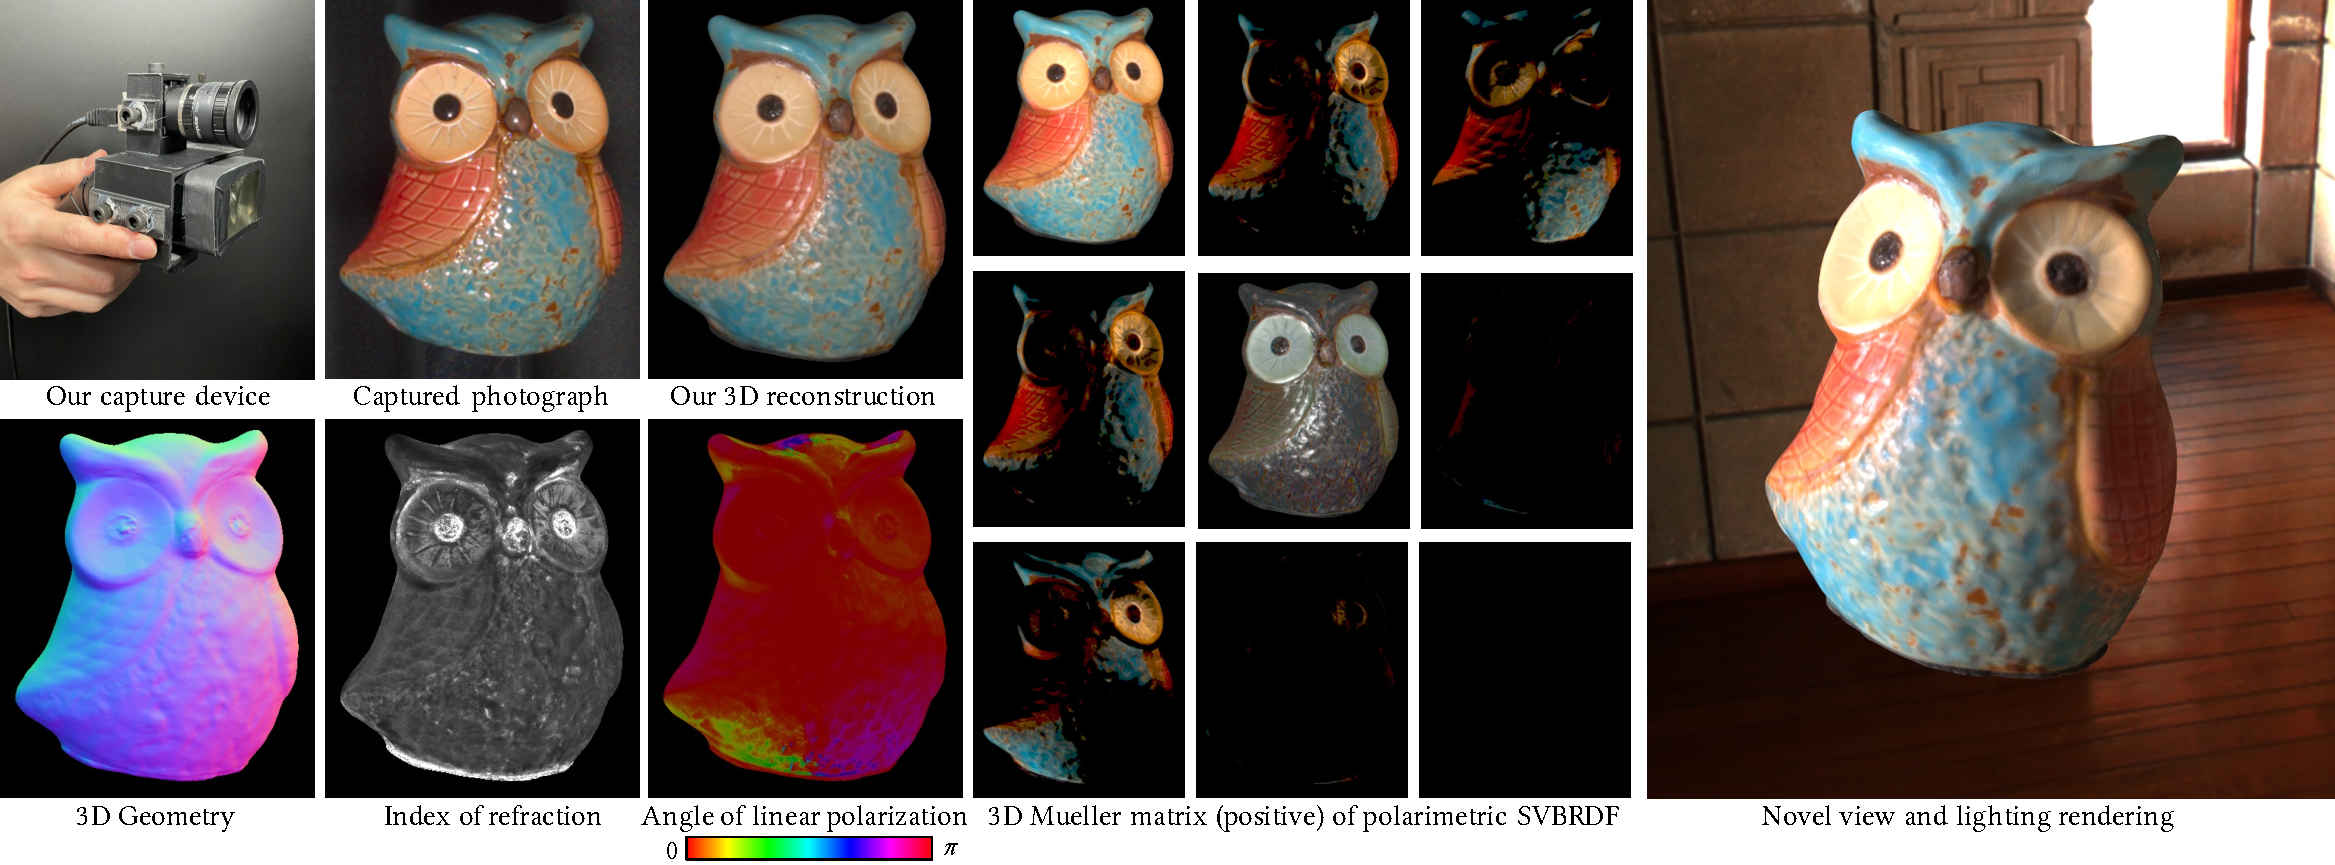
\includegraphics[width=0.95\textwidth]{fig/teaser.pdf}%
	\vspace{-3mm}%
	\caption{본 연구의 촬영 시스템 및 복원 결과물, 3D 뮐러 행렬, 그리고 가상의 시점 및 광원 렌더링 결과물.}
	\label{fig:teaser}
	\vspace{-2mm}
\end{figure*}
%{
%	  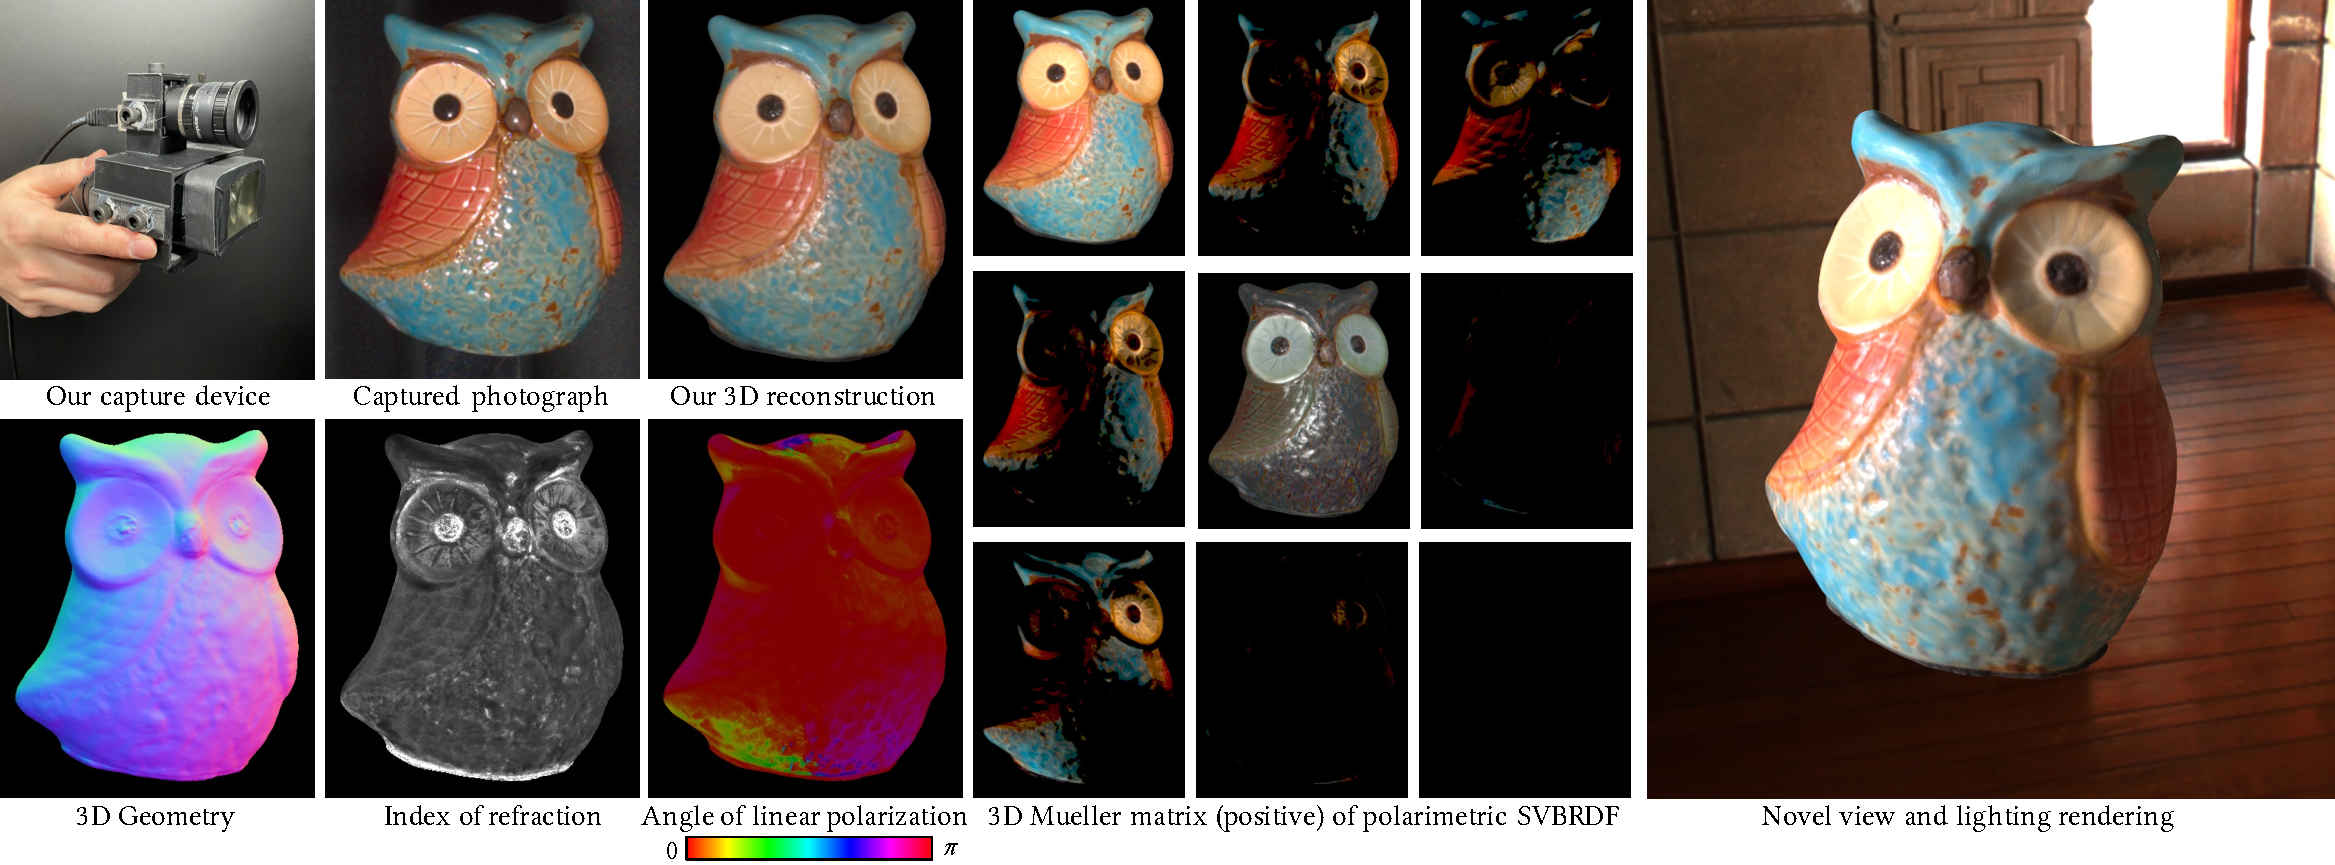
\includegraphics[width=0.95\textwidth]{fig/teaser.pdf}
%	  \caption{본 연구의 촬영 시스템 및 복원 결과물, 3D 뮐러 행렬, 그리고 가상의 시점 및 광원 렌더링 결과물.}
%	  \label{fig:teaser}
%	}

\section{연구 방법}
\label{sec:methods}


\subsection{편광 반사도 모형}
\label{subsec:model}
편광 반사도(pBRDF) 모형은 3가지의 반사 형태로 구성되며, 아래와 같이 표현할 수 있다.
\begin{equation}
	\label{eq:diffuse_and_specular}
	\mathbf{P}={{\mathbf{P}}^{d}}+{{\mathbf{P}}^{s}}+{{\mathbf{P}}^{ss}}.
\end{equation}
${\mathbf{P}}$는 뮐러 행렬로 표현되는 편광 BRDF이며,  ${\mathbf{P}}^{d}$, ${\mathbf{P}}^{s}$ 및 ${\mathbf{P}}^{ss}$는 각각 난반사, 정반사, 단일 산란의 pBRDF이다.
난반사와 정반사의 pBRDF 모형은 Baek et al.\cite{Baek2018}의 모형을 따른다.
%난반사는 빛이 공기에서 매질로 투과 후 여러번의 산란을 거쳐 편광 성분을 모두 잃고, 다시 매질에서 공기로 투과되며 투과에 따른 프레넬 효과를 통해 편광 성분을 갖게 된다.
%정반사는 microfacet 모형을 따르며 각 microfacet 법선에서의 일반적인 반사로서 계산한다.
그러나, 이러한 모델은 단일 산란으로 인하여 편광 성분을 보존한채로 투과되는 경우를 고려하지 못하였다. 
%이러한 단일 산란은 아래의 특성을 갖는다:
%\begin{itemize}
%	\item 단일 산란은 정반사와 비슷한 편광 상태를 갖는다.
%	\item 단일 산란의 거칠기(roughness)는 프레넬 투과와 산란의 위상함수로 만들어진다.
%	\item 정반사는 색깔을 갖지 않으나, 단일 산란은 매질의 흡수에 의한 색을 갖는다.
%\end{itemize}
%위의 관측을 토대로, 인버스 렌더링을 위한 실용적인 단일 산란 모델은 다음과 같다. 
단일 산란의 물리적인 특성을 토대로, 인버스 렌더링을 위한 실용적인 단일 산란 모델은 다음과 같다. 
\begin{equation}
	\label{eq:single_scattering_transport}
	{{\mathbf{P}}^{ss}}= {{\kappa}_{ss}} {{\mathbf{C}}_{h\to o}}\left(-{\varphi_{o}} \right){{\mathbf{F}}^{R}}\left( {{\theta }_{d}};\eta  \right){{\mathbf{C}}_{i\to h}}\left({\varphi_{i}} \right).
\end{equation}
%
$\kappa_{ss}$는 따른 단일 산란 분포 함수, $\mathbf{C}$는 좌표 변환, $\mathbf{F}^{R}$은 프레넬 반사 효과이다.


\subsection{편광 SVBRDF와 기하 구조의 다중 시점 복원}
\label{subsec:reconstruction}

\begin{figure}[tpb]
	\vspace{-2mm}%
	\centering%
	\footnotesize%
	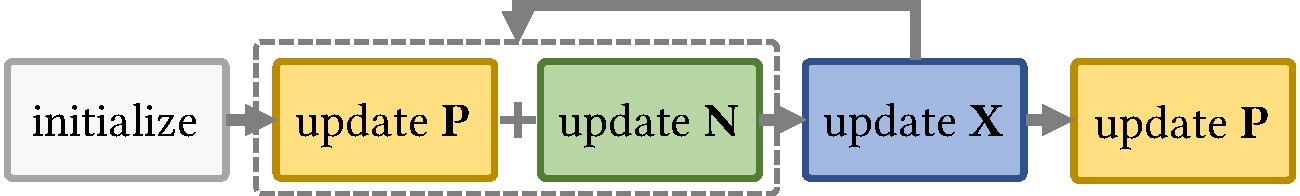
\includegraphics[width=1.0\linewidth]{fig/pipeline-workflow}%
	\vspace{-3mm}%
	\caption{\label{fig:workflow}%
		본 연구 알고리즘의 개요. 편광 SVBRDF $\mathbf{P}$와 쉐이딩 노멀 $\mathbf{N}$의 계산과 3D 기하 구조 $\mathbf{X}$의 복원을 반복적으로 수행한다.
	}
	\vspace{-2mm}
\end{figure}
본 연구 알고리즘의 개요는 Figure~\ref{fig:workflow}와 같다. 먼저 편광 카메라를 포함하는 촬영 시스템을 통해 여러 시점에서 편광 플래시라이트 이미지를 얻는다. 촬영 시스템은 Figure~\ref{fig:teaser}에서 확인할 수 있다.
이를 입력 데이터로 하여 편광 SVBRDF와 쉐이딩 노멀의 계산과 3D 기하 구조의 복원을 반복적으로 수행한다. 
3D 기하 구조의 복원에는 푸아송 표면 재건을\cite{kazhdan2013screened} 이용한다.
편광 SVBRDF와 쉐이딩 노멀의 계산에서는 4가지 로스로 구성된 아래의 최적화를 진행한다.
%\begin{equation}
%	\label{eq:optimization}
%	{\min}_{\eta,\sigma_{s},\rho_s,{\rho}_{ss},{\rho_d},\mathbf{n}}\left( {{\lambda }_{1}}{{\mathcal{L}}_{\psi}}+{{\lambda }_{2}}{{\mathcal{L}}_{d}}+{{\lambda }_{3}}{{\mathcal{L}}_{s}}+{{\lambda }_{4}}{{\mathcal{L}}_{\phi}} \right),
%\end{equation}
\begin{equation}
	\label{eq:optimization}
	{\min}\left( {{\lambda }_{1}}{{\mathcal{L}}_{\psi}}+{{\lambda }_{2}}{{\mathcal{L}}_{d}}+{{\lambda }_{3}}{{\mathcal{L}}_{s}}+{{\lambda }_{4}}{{\mathcal{L}}_{\phi}} \right).
\end{equation}
%
${{\mathcal{L}}_{\psi}}$, ${{\mathcal{L}}_{d}}$, ${{\mathcal{L}}_{s}}$, ${{\mathcal{L}}_{\phi}}$는 각각 굴절률, 난반사, 정반사 및 단일 산란, 그리고 노멀에 대한 로스 함수이다.
정반사의 경우 촬영시의 샘플이 상대적으로 부족하다. 이를 해결하기 위해 두 단계의 정반사 증강 방법을 이용한다.
먼저 비슷한 표면끼리 클러스터링을 이용하여 모델 파라미터를 만든다. 그 다음 가상 샘플들을 생성하여 함께 최적화에 사용한다.
모델과 최적화의 자세한 내용은 원 논문에서 확인할 수 있다.~\cite{Ellipsometry:SIG:2022}


\section{결과}
\label{sec:results}
기존 편광 BRDF 측정 데이터를 이용하여 제안한 모델과 알고리즘을 검증하였다. 또한, Figure~\ref{fig:teaser}와 같이 실제 오브젝트에서 기하 구조, 3D 뮐러 행렬을 취득하였으며 이를 이용하여 가상의 시점 및 광원 렌더링 결과물을 획득하였다.
해당 검증 및 결과의 전체 내용은 원 논문에서 확인할 수 있다.

\section{결론}
\label{sec:conclusion}

본 연구의 sparse ellipsometry 기술을 높은 정확도로 물체의 형상과 편광 SVBRDF를 동시에 측정할 수 있게 해준다. 이는 현존하는 편광해석법에 비해 적은 시간을 이용하며, 손으로 들 수 있는 고정된 광학 요소만을 포함한 장비를 통해 취득할 수 있게 한다. 또한 본 연구는 단일 산란을 포함하는 새로운 pBRDF 모형을 제안하였다. 본 연구는 휴대용 장치를 사용하는 새로운  편광 이미징 응용 방법의 개발을 촉진할 것으로 기대한다. 

%\section*{감사의 글}
%
%감사의 글은 논문의 끝에 번호 없이 작성한다.

%---------------------------------------------------------------------------
% references

\bibliographystyle{IEEEtran}
\nocite{*}
\bibliography{ref}

%---------------------------------------------------------------------------
% done

\end{document}
